\begin{frame}[t]{Multigroup Approximation}


\begin{itemize}
    \item Define multigroup flux and cross sections:
\begin{subequations}
    \begin{equation*}\scriptstyle
    \varphi_g\left(\bm x,\bm \Omega\right)= \intop_{E_n}^{E_{n-1}} \varphi\left(\bm x,E,\bm\Omega\right) dE\ ,
    \end{equation*}
    \begin{equation*}\scriptstyle
    \Sigma_{x,g} \varphi_g =  \intop_{E_n}^{E_{n-1}} \varphi\left(E\right) \Sigma_x\left(E\right) dE \Rightarrow \Sigma_x,g = \frac{\intop_{E_n}^{E_{n-1}} \varphi\left(E\right) \Sigma_x\left(E\right)\ . dE}{\intop_{E_n}^{E_{n-1}} \varphi\left(E\right) dE}
    \end{equation*}
\end{subequations}
\item Operate on steady-state transport equation by $\intop_{E_n}^{E_{n-1}}\left(\cdot\right)dE$
\end{itemize}

\begin{center}
    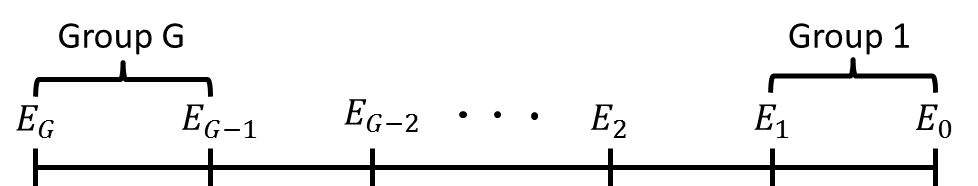
\includegraphics[width=0.8\textwidth]{MGillustration.png}
\end{center}

\end{frame}

%%%%%%%%%%%%%%%%%%%%%%%%%%%%%%%%%%%%%%%%%%%%%%%%%%%%%%%%%%%%%%%%%%%%%%%%%%%%%%%%

\begin{frame}[t]{Angle Discretization}

\begin{itemize}
    \item Select a set of azimuthal and polar angles $\alpha$ and $\mu$
\begin{align*}\scriptstyle
\bm\Omega &= \cos\left(\alpha\right)\sqrt{1-\mu^2}\bm i + \sin\left(\alpha\right)\sqrt{1-\mu^2}\bm j + \mu\bm k \\
\Rightarrow \bm\Omega_n &= \cos\left(\alpha_n\right)\sqrt{1-\mu_n^2}\bm i + \sin\left(\alpha_n\right)\sqrt{1-\mu_n^2}\bm j + \mu_n\bm k\ .
\end{align*}
\item A quadrature can be used with weights $w_n$ associated with each angle $\Omega_n$
\begin{subequations}
    \begin{equation*}\scriptstyle
    \intop d\Omega = \sum_{n=1}^N w_n = 4\pi\ ,
    \end{equation*}
    \begin{equation*}\scriptstyle
    \intop \bm\Omega d\Omega = \sum_{n=1}^N \bm\Omega_n w_n = 0\ ,
    \end{equation*}
    \begin{equation*}\scriptstyle
    \intop_{4\pi} f\left(\bm\Omega\right)d\Omega \approx \sum_{n=1}^N f_n w_n\ .
    \end{equation*}
\end{subequations}
\end{itemize}

\end{frame}

%%%%%%%%%%%%%%%%%%%%%%%%%%%%%%%%%%%%%%%%%%%%%%%%%%%%%%%%%%%%%%%%%%%%%%%%%%%%%%%%

\begin{frame}[t]{Transport-Corrected Scattering Approximation}

\begin{itemize}
\item Modifies self-scatter and total cross-sections to account for 
anisotropy while performing isotropic calculations
\item Neutron Leakage Conservation (NLC) Method: H-1
\begin{equation*}
\Sigma_{s0,g\rightarrow g} = \Sigma_{s0,g\rightarrow g} + \frac{1}{3D_g} 
- \Sigma_{t,g}
\end{equation*}
\item In-Scatter Method: B-11, C-12, O-16
\begin{equation*}
\Sigma_{s0,g\rightarrow g} = \Sigma_{s0,g\rightarrow g} - 
\frac{1}{\phi_{1,g}}\sum_{g'=1}^G \Sigma_{s1,g'\rightarrow g}\phi_{1,g'}
\end{equation*}
\item Out-Scatter Method: All other isotopes
\begin{equation*}
\Sigma_{s0,g\rightarrow g} = \Sigma_{s0,g\rightarrow g} - \sum_{g'=1}^G 
\Sigma_{s1,g\rightarrow g'}
\end{equation*}
\end{itemize}

\end{frame}

%%%%%%%%%%%%%%%%%%%%%%%%%%%%%%%%%%%%%%%%%%%%%%%%%%%%%%%%%%%%%%%%%%%%%%%%%%%%%%%%

\begin{frame}[t]{Collision Probabilities}

\begin{itemize}
    \item Used to calculate flux spectra in a pin cell
    \item Transport equation written so right-hand side is a single source term
    \begin{itemize}
        \item Assumes only scattering and fission sources
        \item Assumes isotropic scattering
    \end{itemize}
    \item For 1D, pin cell is discretized into $R$ rings, assuing flat source, flux, and cross section in each ring
    \item A matrix with elements $T_{g,r' \rightarrow r}$ can be determined
    \begin{itemize}
        \item Each element is probability of neutron born in group $g$ and region $r'$ reaching region $r$
        \item These probabilities are geometry-dependent, but have a general form for 1D cylindrical geometry
    \end{itemize}
    \item Flux in each ring can be calculated from matrix $\bm T$, sources $q$, and volumes $V$
\begin{equation*}\scriptstyle
\phi_{g,r} = \sum_{r'=1}^R T_{g,r'\rightarrow r} q_{g,r'} V_{r'}
\end{equation*}
\end{itemize}

\end{frame}

%%%%%%%%%%%%%%%%%%%%%%%%%%%%%%%%%%%%%%%%%%%%%%%%%%%%%%%%%%%%%%%%%%%%%%%%%%%%%%%%%

\begin{frame}
\begin{center}
\resizebox{0.5\textwidth}{!}{\begin{tikzpicture}[node distance=2cm]

% Start
\node (start) [startstop] {Start};

% CMFD
\node (homog) [process, right of=start, xshift=2.0cm] {Homogenize Cross-sections and Flux; Calculate $\tilde{D}$};
\node (iterCheck) [decision, below of=homog, yshift=-1.5cm] {First Iteration?};
\node (firstIter) [process, below of=iterCheck, xshift=-2.5cm, yshift=-1.0cm] {Set $\hat{D}=0$};
\node (laterIter) [process, below of=iterCheck, xshift=2.5cm, yshift=-1.0cm] {Calculate $\hat{D}$};
\node (matrix) [process, below of=firstIter, xshift=2.5cm] {Set up CMFD Matrix};
\node (3DCMFD) [process, below of=matrix] {3D CMFD Calculation};
\node (proj) [process, below of=3DCMFD] {Scale MOC flux with CMFD flux};

% Stop
\node (stop) [startstop, right of=proj, xshift=2.0cm] {Stop};

% Basic Arrows
\draw [arrow] (start) -- (homog);
\draw [arrow] (homog) -- (iterCheck);
\draw [arrow] (matrix) -- (3DCMFD);
\draw [arrow] (3DCMFD) -- (proj);
\draw [arrow] (proj) -- (stop);

% Fancy Arrows
\draw [arrow] (iterCheck) -| node[anchor=south] {yes} (firstIter);
\draw [arrow] (iterCheck) -| node[anchor=south] {no} (laterIter);
\draw [arrow] (firstIter) |- (matrix);
\draw [arrow] (laterIter) |- (matrix);

\end{tikzpicture}}
\end{center}
\end{frame}

%%%%%%%%%%%%%%%%%%%%%%%%%%%%%%%%%%%%%%%%%%%%%%%%%%%%%%%%%%%%%%%%%%%%%%%%%%%%%%%%%

\begin{frame}
\begin{center}
\resizebox{0.6\textwidth}{!}{\begin{tikzpicture}[node distance=2cm]

% Begin
\node (start) [startstop] {Start};

% Nodal
\node (radialTL) [process, right of=start, xshift=2.5cm] {Calculate radial transverse leakage source};
\node (sp3-0) [process, below of=radialTL] {Solve 0th moment equation};
\node (sp3-2) [process, below of=sp3-0] {Solve 2nd moment equation};
\node (convCheck) [decision, below of=sp3-2, yshift=-1.5cm] {Converged?};

% Stop
\node (stop) [startstop, right of=convCheck, xshift=2.5cm] {Stop};

% Basic Arrows
\draw [arrow] (start) -- (radialTL);
\draw [arrow] (radialTL) -- (sp3-0);
\draw [arrow] (sp3-0) -- (sp3-2);
\draw [arrow] (sp3-2) -- (convCheck);
\draw [arrow] (convCheck) -- node[anchor=north] {yes} (stop);

% Fancy Arrows
\draw [arrow] (convCheck) -| node[anchor=north] {no} ([xshift=-1.5cm]sp3-2.west) |- (sp3-0);

\end{tikzpicture}}
\end{center}
\end{frame}

%%%%%%%%%%%%%%%%%%%%%%%%%%%%%%%%%%%%%%%%%%%%%%%%%%%%%%%%%%%%%%%%%%%%%%%%%%%%%%%%%

\begin{frame}
\begin{center}
\resizebox{0.5\textwidth}{!}{\begin{tikzpicture}[node distance=2cm]

% Begin
\node (start) [startstop] {Start};
\node (init) [io, right of=start, xshift=2.5cm] {Input N$_{inners}$};

% MOC
\node (begin) [process, below of=init] {Set $n=0$};
\node (source) [process, below of=begin] {Calculate fission and axial transverse leakage sources};
\node (scatSource) [process, below of=source] {Calculate scattering source};
\node (MOC) [process, below of=scatSource] {2D MOC sweep over each energy group};
\node (MOCdone) [decision, below of=MOC, yshift=-1.5cm] {$n = N_{inners}$?};z
\node (stop) [startstop, right of=MOCdone, xshift=2.5cm] {Stop};

% Basic Arrows
\draw [arrow] (start) -- (init);
\draw [arrow] (init) -- (begin);
\draw [arrow] (begin) -- (source);
\draw [arrow] (source) -- (scatSource);
\draw [arrow] (scatSource) -- (MOC);
\draw [arrow] (MOC) -- (MOCdone);

% Fancy Arrows
\draw [arrow] (MOCdone) -| node[anchor=north] {no} ([xshift=-1.5cm]MOC.west) |- (scatSource);
\draw [arrow] (MOCdone) -- node[anchor=north] {yes} (stop);

\end{tikzpicture}}
\end{center}
\end{frame}

%%%%%%%%%%%%%%%%%%%%%%%%%%%%%%%%%%%%%%%%%%%%%%%%%%%%%%%%%%%%%%%%%%%%%%%%%%%%%%%%%

\begin{frame}
\vspace{-10pt}
\begin{center}
\resizebox{0.4\textwidth}{!}{\begin{tikzpicture}[node distance=2cm]

% Start
\node (start) [startstop] {Start};

% CMFD
\node (homog) [process, right of=start, xshift=2.0cm] {Homogenize cross-sections and flux; Calculate $\tilde{D}$};
\node (1dcpm) [process, below of=start, yshift=-0.5cm] {1D CP calculations};
\node (homogCP) [process, right of=1dcpm, xshift=2.0cm] {Re-homogenize cross-sections in partially rodded pin cells};
\node (iterCheck) [decision, below of=homogCP, yshift=-1.5cm] {First iteration?};
\node (firstIter) [process, below of=iterCheck, xshift=-2.5cm, yshift=-1.0cm] {Set $\hat{D}=0$};
\node (laterIter) [process, below of=iterCheck, xshift=2.5cm, yshift=-1.0cm] {Calculate $\hat{D}$};
\node (matrix) [process, below of=firstIter, xshift=2.5cm] {Set up CMFD matrix};
\node (3DCMFD) [process, below of=matrix] {3D CMFD calculation};
\node (proj) [process, below of=3DCMFD] {Scale MOC flux with CMFD flux};
\node (projCP) [process, below of=proj] {Homogenize partially rodded MOC cross-sections};

% Stop
\node (stop) [startstop, right of=projCP, xshift=2.0cm] {Stop};

% Basic Arrows
\draw [arrow] (start) -- (homog);
\draw [arrow] (1dcpm) -- (homogCP);
\draw [arrow] (homogCP) -- (iterCheck);
\draw [arrow] (matrix) -- (3DCMFD);
\draw [arrow] (3DCMFD) -- (proj);
\draw [arrow] (proj) -- (projCP);
\draw [arrow] (projCP) -- (stop);

% Fancy Arrows
\draw [arrow] (homog) |- ([yshift=-0.75cm]start.south) -| (1dcpm);
\draw [arrow] (iterCheck) -| node[anchor=south] {yes} (firstIter);
\draw [arrow] (iterCheck) -| node[anchor=south] {no} (laterIter);
\draw [arrow] (firstIter) |- (matrix);
\draw [arrow] (laterIter) |- (matrix);

\end{tikzpicture}}
\end{center}
\end{frame}

%%%%%%%%%%%%%%%%%%%%%%%%%%%%%%%%%%%%%%%%%%%%%%%%%%%%%%%%%%%%%%%%%%%%%%%%%%%%%%%%%

\begin{frame}[t]{2D/3D}

\begin{itemize}
    \item 2D MOC is used to generate homogenized cross sections
    \item MOC planes are homogenized onto Cartesian grid
    \item 3D S$_N$ is used to solve the 3D transport equation on the homogenized coarse mesh
\end{itemize}
\begin{center}
    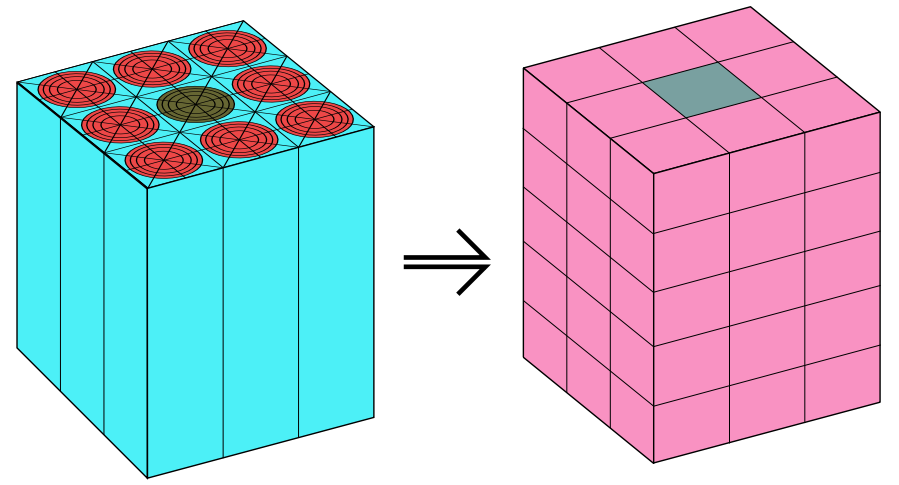
\includegraphics[width=0.7\textwidth]{2d-3d.png}
\end{center}

\end{frame}

%%%%%%%%%%%%%%%%%%%%%%%%%%%%%%%%%%%%%%%%%%%%%%%%%%%%%%%%%%%%%%%%%%%%%%%%%%%%%%%%

\begin{frame}[t]{1D MOC}

\begin{itemize}
    \item 1D MOC code developed that uses MOC cross sections and slab geometry
    \item Fixed source and eigenvalue calculations both supported
    \item Analysis of angular flux behavior for cross section mixtures could be performed
\end{itemize}
\begin{center}
    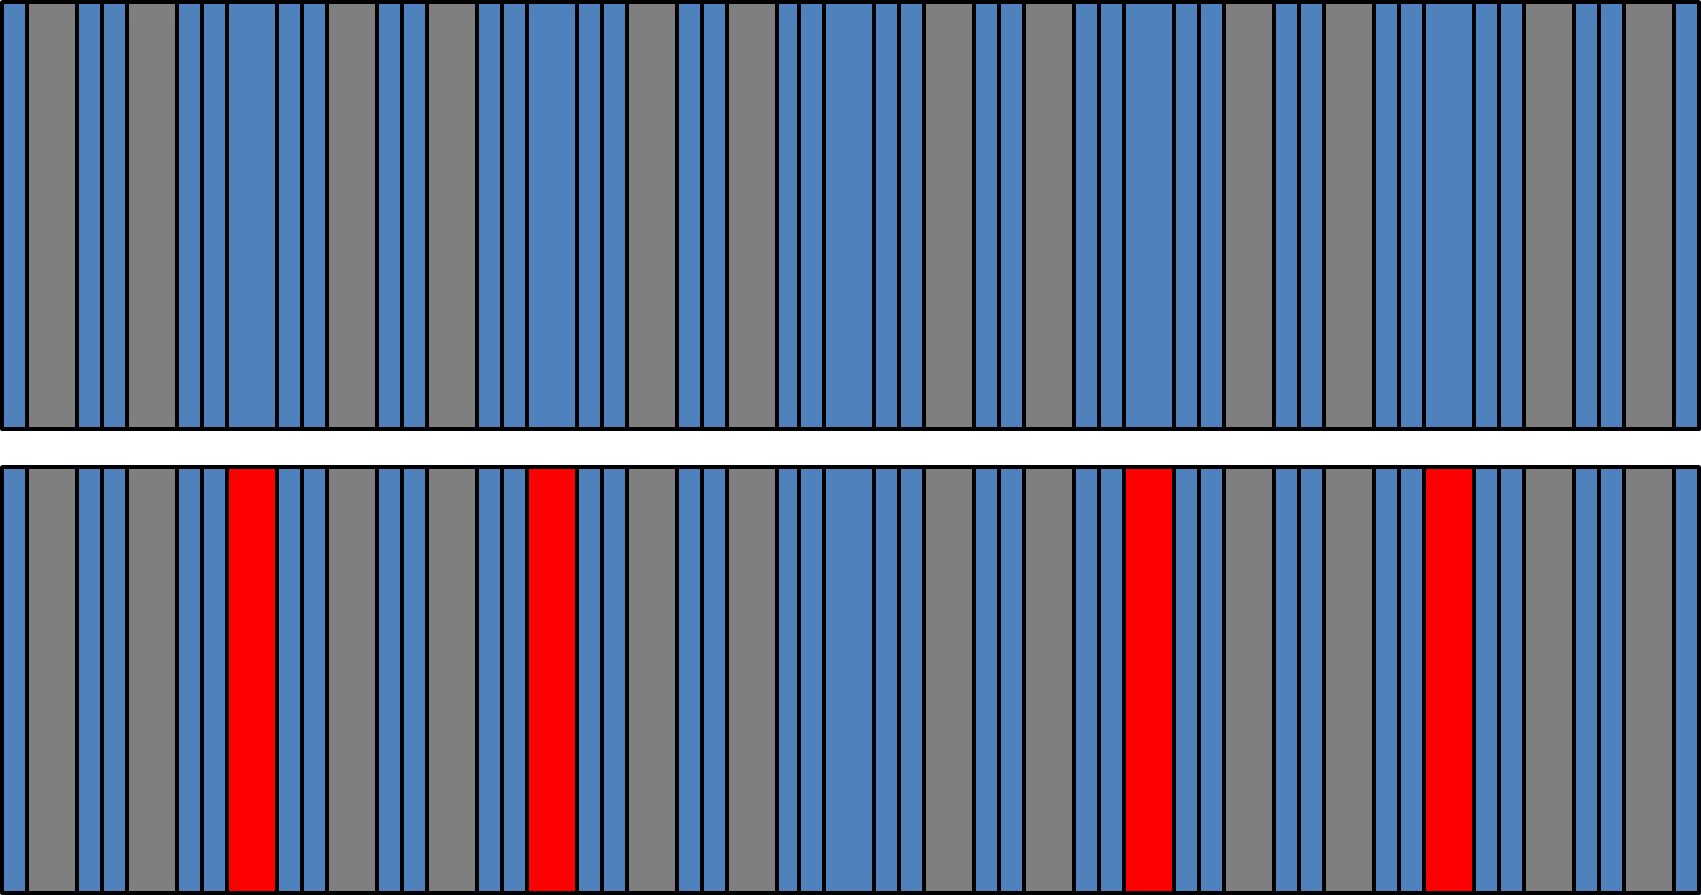
\includegraphics[width=0.6\textwidth]{1dmoc-3x17-geom.png}
\end{center}

\end{frame}

%%%%%%%%%%%%%%%%%%%%%%%%%%%%%%%%%%%%%%%%%%%%%%%%%%%%%%%%%%%%%%%%%%%%%%%%%%%%%%%%

\begin{frame}[t]{1D MOC -- Fixed Total Source}

\begin{itemize}
    \item Scalar flux, group 7
\end{itemize}
\begin{center}
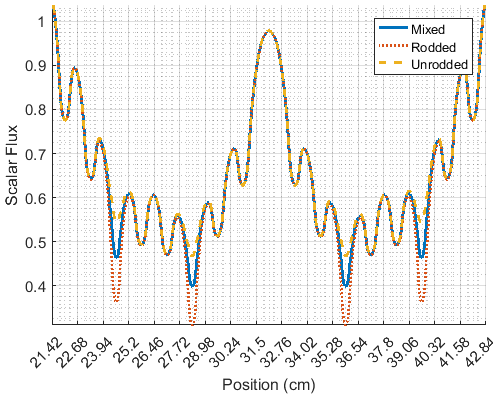
\includegraphics[width=0.5\textwidth]{1dmoc-50mix-fixedscat-scalflux7.png}
\end{center}

\end{frame}

%%%%%%%%%%%%%%%%%%%%%%%%%%%%%%%%%%%%%%%%%%%%%%%%%%%%%%%%%%%%%%%%%%%%%%%%%%%%%%%%

\begin{frame}[t]{1D MOC -- Fixed Total Source}

\begin{itemize}
    \item Rightgoing angular flux, group 1 (left) and 7 (right)
\end{itemize}

\begin{center}
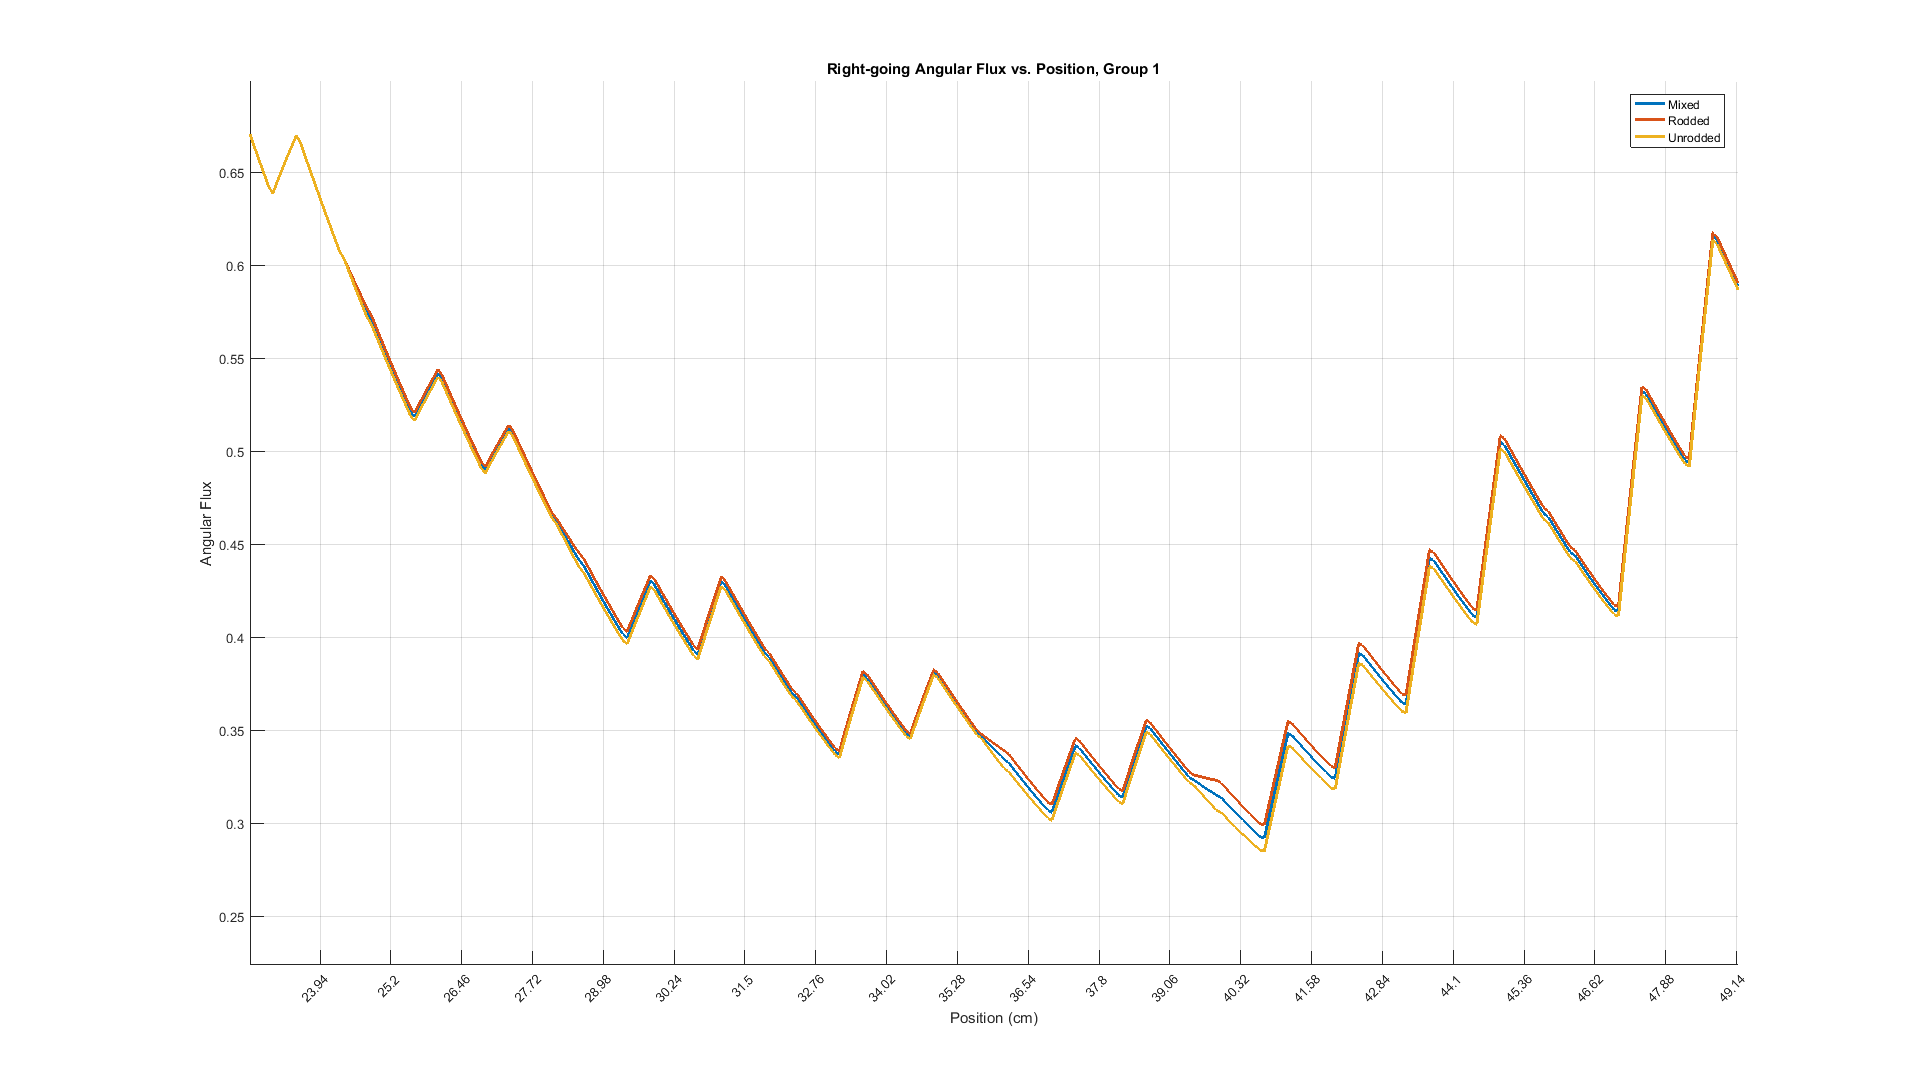
\includegraphics[width=0.45\textwidth]{1dmoc-50mix-fixedscat-angflux1.png} 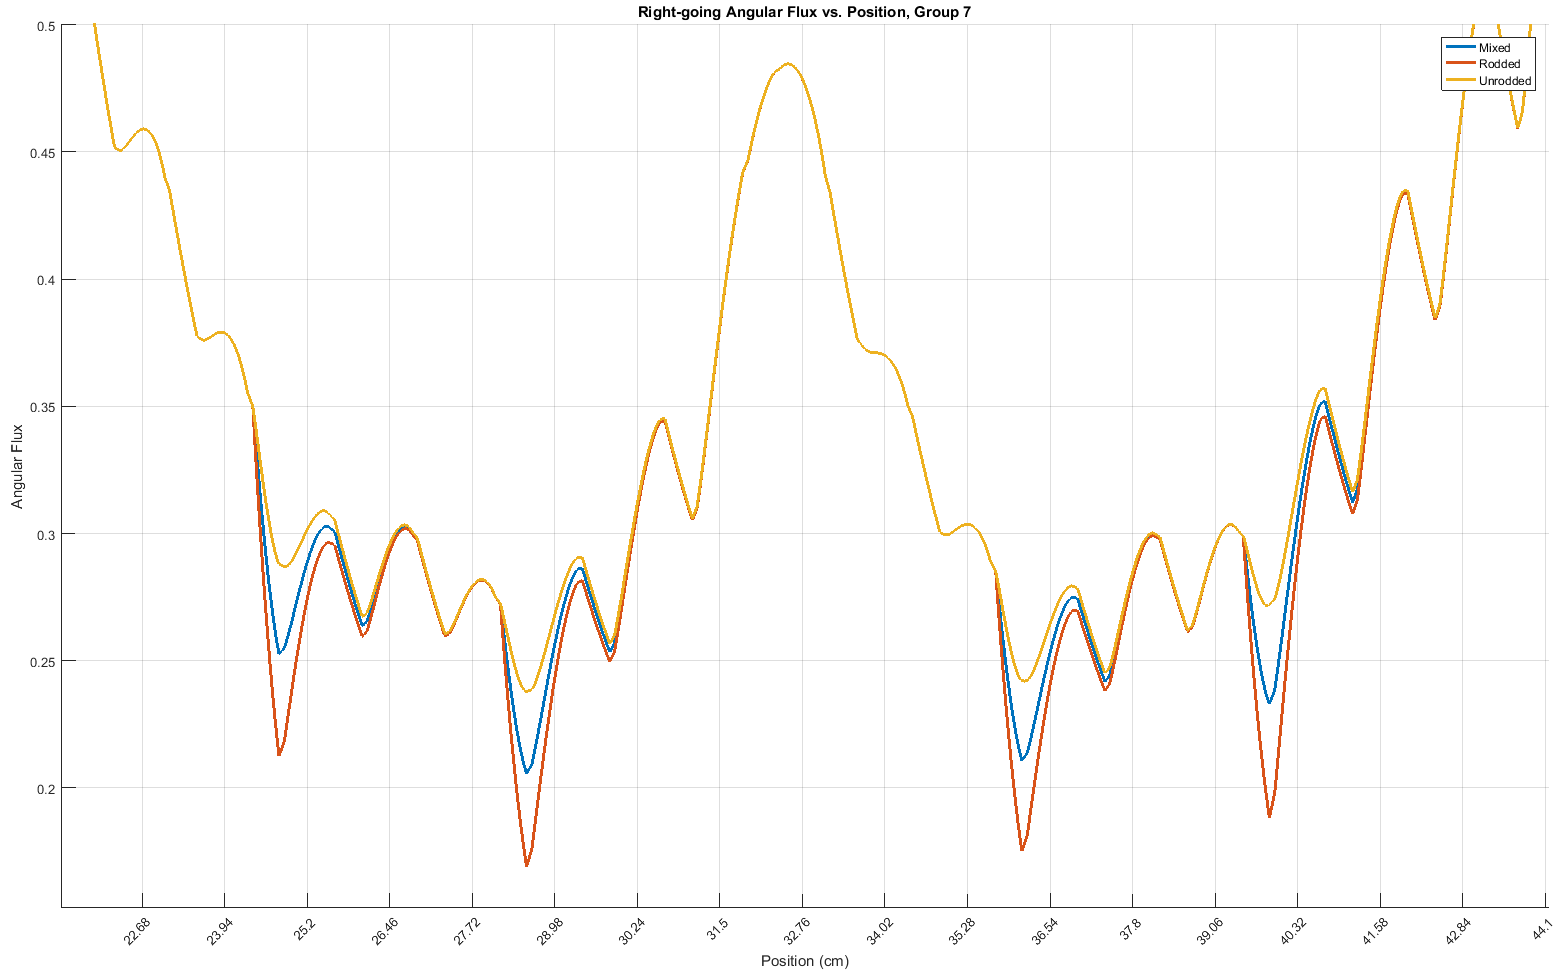
\includegraphics[width=0.45\textwidth]{1dmoc-50mix-fixedscat-angflux7.png}
\end{center}

\end{frame}

%%%%%%%%%%%%%%%%%%%%%%%%%%%%%%%%%%%%%%%%%%%%%%%%%%%%%%%%%%%%%%%%%%%%%%%%%%%%%%%%

\begin{frame}[t]{1D MOC -- Fixed Fission Source}

\begin{itemize}
    \item Rightgoing angular flux, group 1 (left) and 7 (right)
\end{itemize}
\begin{center}
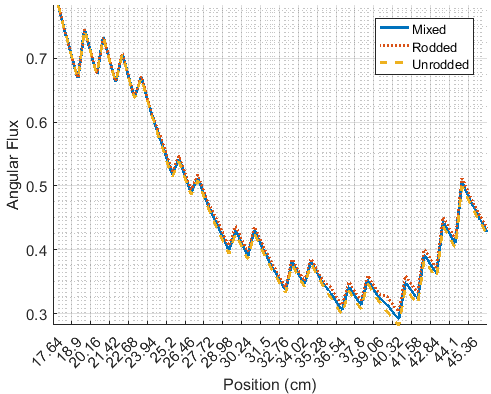
\includegraphics[width=0.45\textwidth]{1dmoc-50mix-angflux1.png} 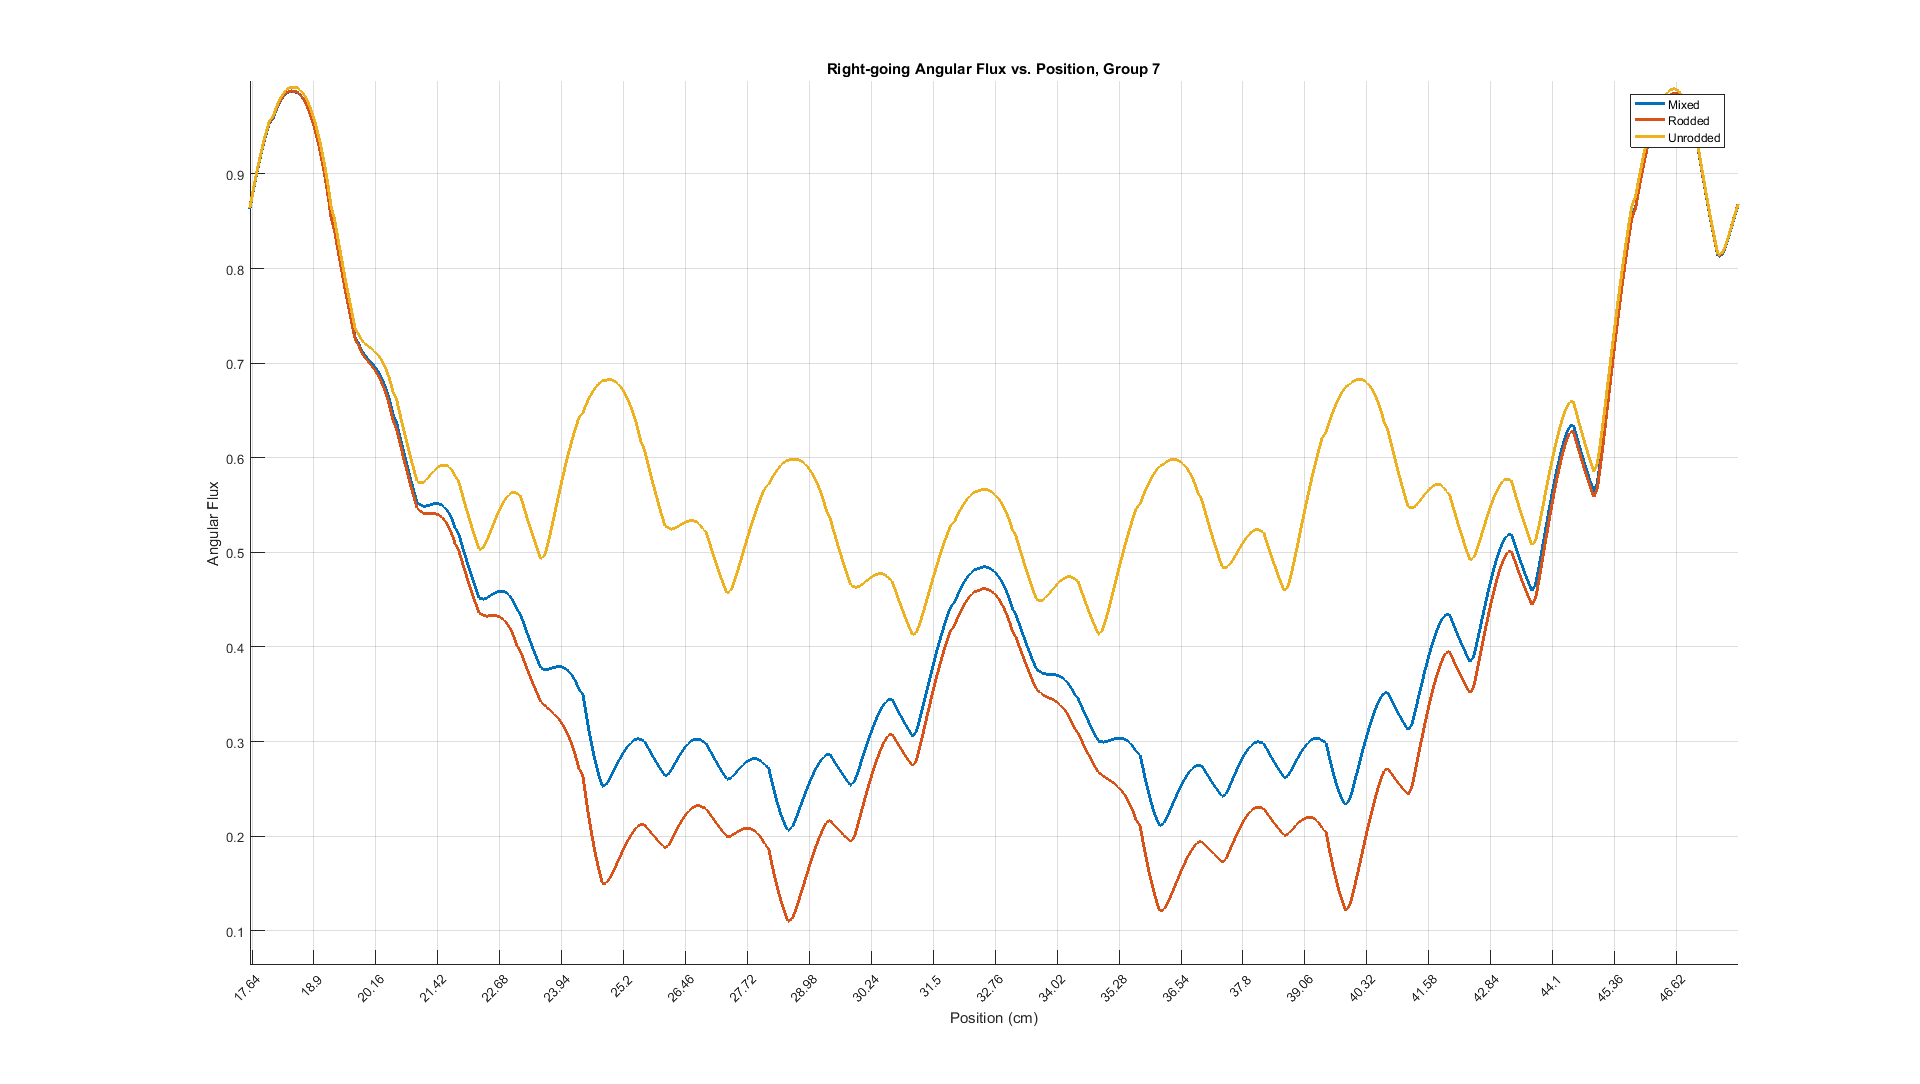
\includegraphics[width=0.45\textwidth]{1dmoc-50mix-angflux7.png}
\end{center}

\end{frame}

%%%%%%%%%%%%%%%%%%%%%%%%%%%%%%%%%%%%%%%%%%%%%%%%%%%%%%%%%%%%%%%%%%%%%%%%%%%%%%%%

\begin{frame}[t]{1D Subray MOC}

\begin{itemize}
    \item 1D MOC code developed that uses MOC cross sections and slab geometry
    \item Fixed source and eigenvalue calculations both supported
    \item Allowed for a prototype of subray MOC concept
\end{itemize}
\begin{center}
    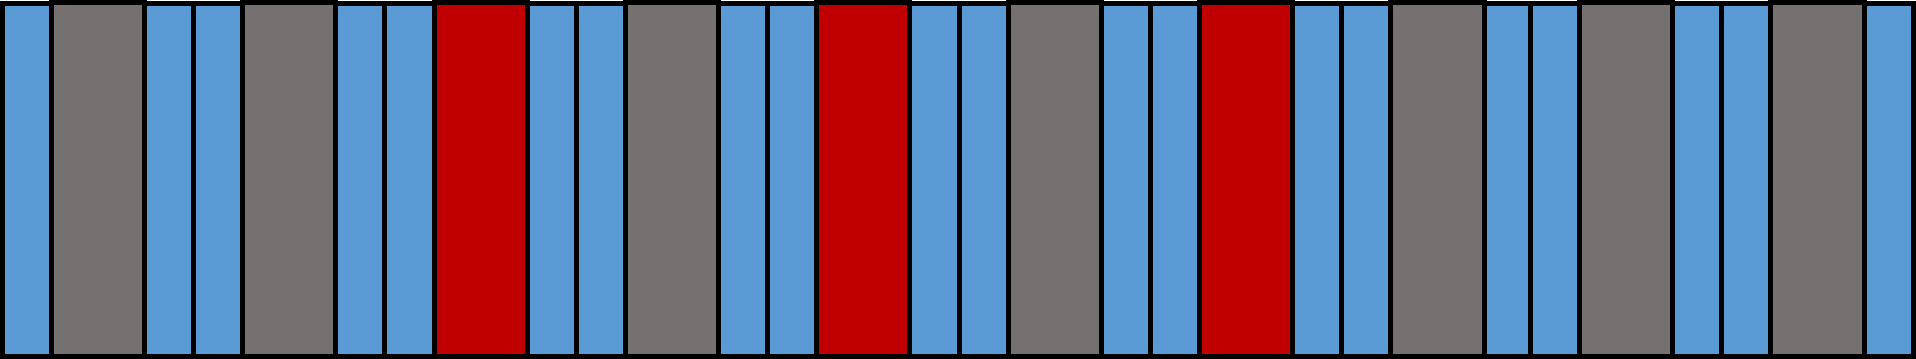
\includegraphics[width=0.8\textwidth]{10pin-slab-geometry.png}
\end{center}

\end{frame}

%%%%%%%%%%%%%%%%%%%%%%%%%%%%%%%%%%%%%%%%%%%%%%%%%%%%%%%%%%%%%%%%%%%%%%%%%%%%%%%%

\begin{frame}[t]{1D Subray MOC}

\begin{center}
    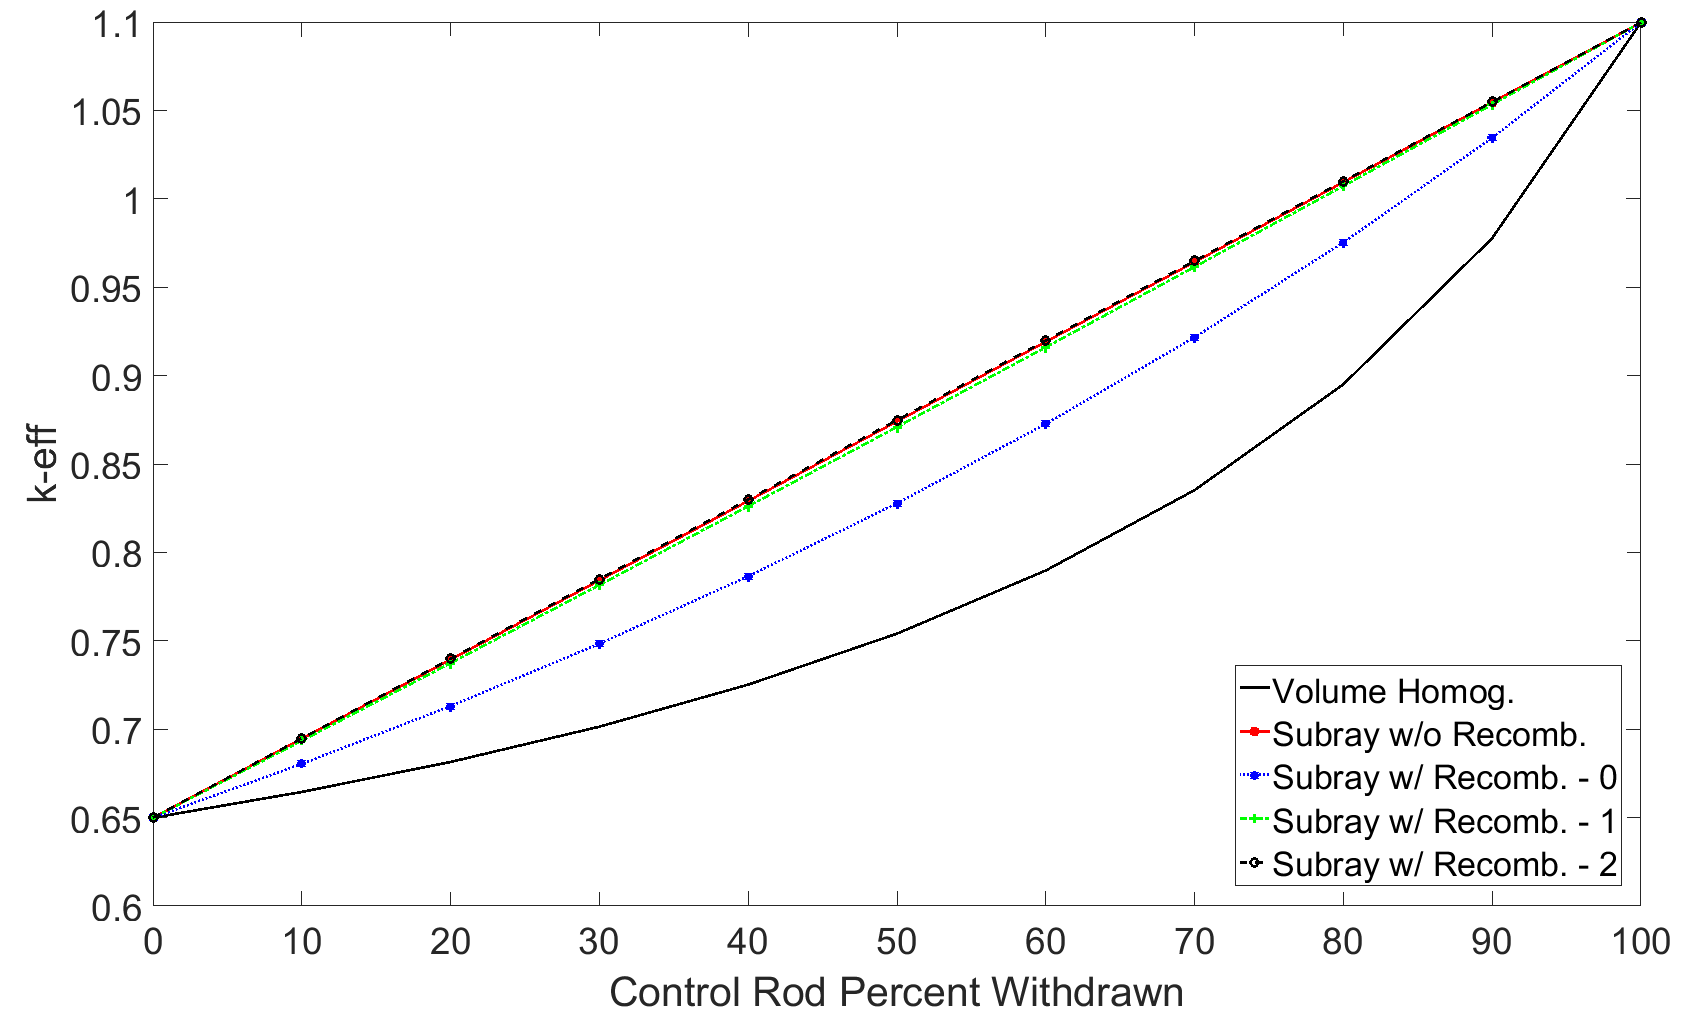
\includegraphics[width=0.8\textwidth]{keff_subray.png}
\end{center}

\end{frame}

%%%%%%%%%%%%%%%%%%%%%%%%%%%%%%%%%%%%%%%%%%%%%%%%%%%%%%%%%%%%%%%%%%%%%%%%%%%%%%%%

\begin{frame}[t]{1D Subray MOC}

\begin{itemize}
    \item 50\% rodded, scalar flux, group 1
\end{itemize}
\begin{center}
    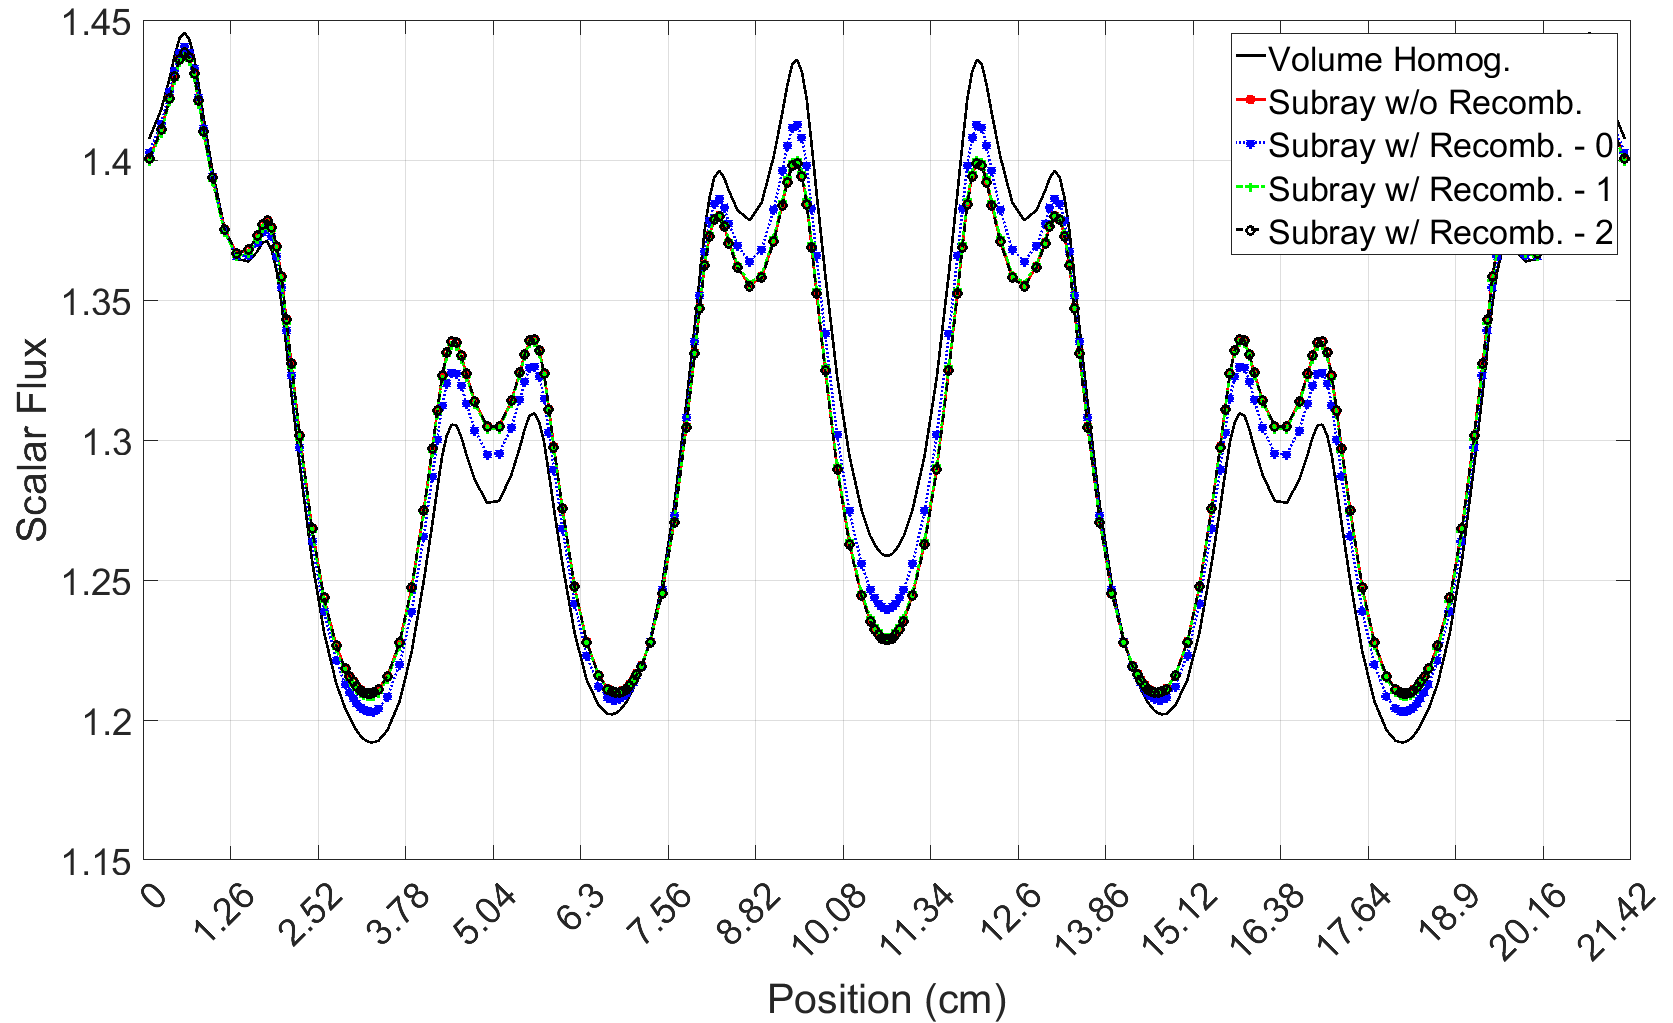
\includegraphics[width=0.8\textwidth]{scalflux1.png}
\end{center}

\end{frame}

%%%%%%%%%%%%%%%%%%%%%%%%%%%%%%%%%%%%%%%%%%%%%%%%%%%%%%%%%%%%%%%%%%%%%%%%%%%%%%%%

\begin{frame}[t]{1D Subray MOC}

\begin{itemize}
\item 50\% rodded, scalar flux, group 7
\end{itemize}
\begin{center}
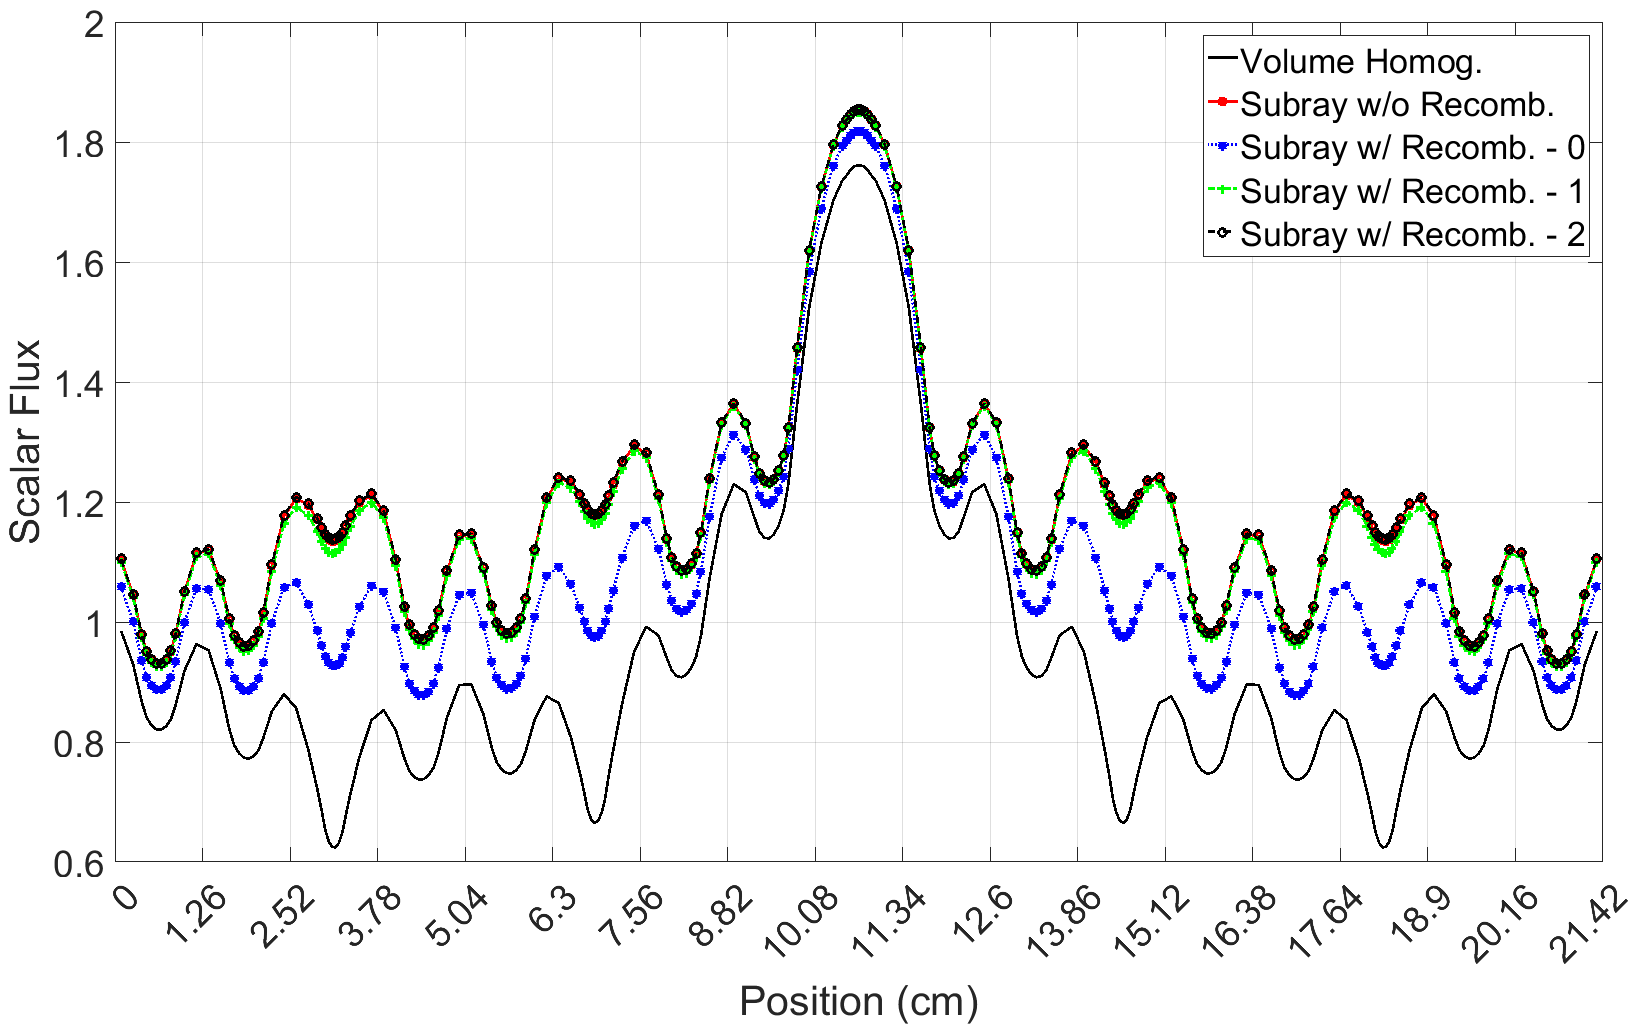
\includegraphics[width=0.8\textwidth]{scalflux7.png}
\end{center}

\end{frame}